\section{The Kitaev-Heisenberg Model} 
\todo{Maybe making this a section is kinda unnecessary?}

\begin{figure*}[t]
    \centering
    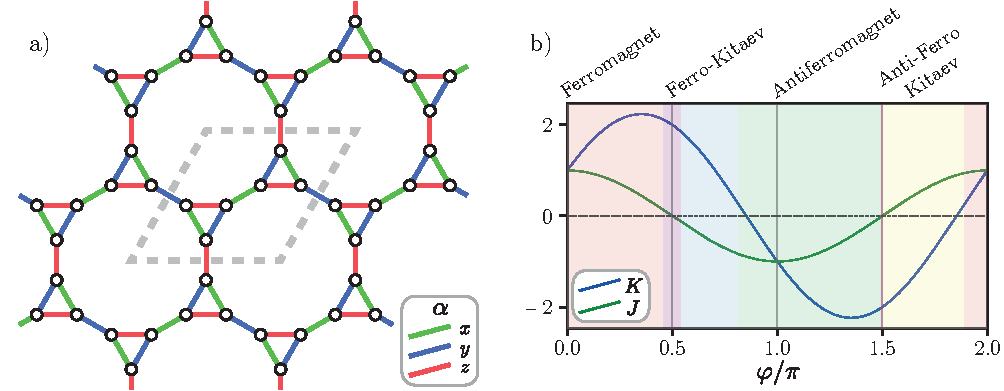
\includegraphics[]{kitaev_heisenberg_star/figures/star_lattice.pdf}
    \caption{ 
        \textbf{(a)} A fragment of the star lattice is shown. Bond labelling is indicated by the colouring, and the six-site unit cell is depicted with a grey dashed rhombus.
        \textbf{(b)} The dependence of the $J$ and $K$ values on the parameter $\varphi$ is shown. The two pure Heisenberg and two pure Kitaev points are labelled. The background colouring corresponds to the phase boundaries obtained in \textsection\ref{sec:dmrg}.
     }
    \label{fig:star_lattice_and_jk}
\end{figure*}

Let us start by defining the model, which we shall construct on the star lattice shown in fig.~\ref{fig:star_lattice_and_jk}a. As in the previous chapter, each site hosts a single spin-1/2, and bonds are coloured with a label $\alpha \in \{x,y,z\}$ such that no vertex touches two bonds of the same colour.
%
We choose the Hamiltonian to interpolate between two well-studied limits: the spin isotropic Heisenberg and the anisotropic Kitaev limit, where each bond of type $\alpha$ is coupled only in the direction that matches the colouring: 
\begin{align} \label{eqn:kitave_heisenberg_hamiltonian}
    H = -
    \sum_{\braket{jk}_\alpha } \bigg (  K \sigma_j^\alpha \sigma_k^\alpha
    +J \sum_{\bar \alpha \neq \alpha}  \sigma_j^{\bar \alpha} \sigma_k^{\bar \alpha}
    \bigg ).
\end{align}
Here $\braket{jk}_\alpha$ indicates a bond of type $\alpha$ that connects adjacent sites $j$ and $k$. The parameter $K$ determines the strength of the ``on-colouring'' coupling, where the coupling direction matches $\alpha$, and $J$ determines the strength of the two remaining ``off-colouring'' couplings. In analogy with previous studies~\cite{chaloupka_zigzag_2013, gohlke_dynamics_2017}, let us introduce a single parameter $\varphi \in [0,2\pi]$ that smoothly maps onto the possibilities for $K$ and $J$ according to
\begin{align} \begin{aligned} \label{eqn:phi_def}
    K &= 2\sin \varphi + \cos \varphi, \\
    J &= \cos \varphi,
\end{aligned}\end{align}
shown in fig.~\ref{fig:star_lattice_and_jk}b. 
% In Appendix~\ref{sec:spin_flip_transformation}, we detail a \textit{four-unit-cell rotation} which, by rotating the axis of a subset spins, maps $J \rightarrow -J$ while leaving $K$ invariant.